\documentclass[12pt,openany,a4paper]{book}
\usepackage{graphics}	% if you want encapsulated PS figures.
\usepackage{graphicx}
\usepackage[colorlinks,allcolors=blue]{hyperref, xcolor} % must be bfore pgfplots
\usepackage{pgfplots} % must be after xcolor
\usepackage{colortbl}
\usepackage{float}
\usepackage{flafter}
% If you use a macro file called macros.tex :
% \input{macros}
% Note: The present document has its macros built in.

% Number subsections but not subsubsections:
\setcounter{secnumdepth}{2}
% Show subsections but not subsubsections in table of contents:
\setcounter{tocdepth}{2}

\pagestyle{headings}		% Chapter on left page, Section on right.
\raggedbottom

\setlength{\topmargin}		{-5mm}  %  25-5 = 20mm7
\setlength{\oddsidemargin}	{10mm}  % rhs page inner margin = 25+10mm
\setlength{\evensidemargin}	{0mm}   % lhs page outer margin = 25mm
\setlength{\textwidth}		{150mm} % 35 + 150 + 25 = 210mm
\setlength{\textheight}		{240mm} % 

\renewcommand{\baselinestretch}{1.2}	% Looks like 1.5 spacing.

% Stop figure/tables smaller than 3/4 page from appearing alone on a page:
\renewcommand{\textfraction}{0.25}
\renewcommand{\topfraction}{0.75}
\renewcommand{\bottomfraction}{0.75}
\renewcommand{\floatpagefraction}{0.75}

% THEOREM-LIKE ENVIRONMENTS:
\newtheorem{defn}	{Definition}	% cf. \dfn for cross-referencing
\newtheorem{theorem}	{Theorem}	% cf. \thrm for cross-referencing
\newtheorem{lemma}	{Lemma}		% cf. \lem for cross-referencing

% AIDS TO CROSS-REFERENCING (All take a label as argument):
\newcommand{\eref}[1] {(\ref{#1})}		% (...)
\newcommand{\eq}[1]   {Eq.\,(\ref{#1})}		% Eq.~(...)
\newcommand{\eqs}[2]  {Eqs.~(\ref{#1}) and~(\ref{#2})}
\newcommand{\dfn}[1]  {Definition~\ref{#1}}	% Definition~...
\newcommand{\thrm}[1] {Theorem~\ref{#1}}	% Theorem~...
\newcommand{\lem}[1]  {Lemma~\ref{#1}}		% Lemma~...
\newcommand{\fig}[1]  {Fig.\,\ref{#1}}		% Fig.~...
\newcommand{\tab}[1]  {Table~\ref{#1}}		% Table~...
\newcommand{\chap}[1] {Chapter~\ref{#1}}	% Chapter~...
\newcommand{\secn}[1] {Section~\ref{#1}}	% Section~...
\newcommand{\ssec}[1] {Subsection~\ref{#1}}	% Subsection~...

% AIDS TO FORMATTING:
\newcommand{\teq}[1]	{\mbox{$#1$}}	% in-Text EQuation (unbreakable)
\newcommand{\qed}	{\hspace*{\fill}$\bullet$}	% end of proof

% MATHEMATICAL TEMPLATES:
% Text or math mode:
\newcommand{\half}	{\ensuremath{\frac{1}{2}}}	% one-half
\newcommand{\halftxt}	{\mbox{$\frac{1}{2}$}}	  	% one-half, small
% Math mode only:
% N.B. Parentheses are ROUND; brackets are SQUARE!
\newcommand{\oneon}[1]	{\frac{1}{#1}}		  % reciprocal
\newcommand{\pow}[2]	{\left({#1}\right)^{#2}}  % Parenthesized pOWer
\newcommand{\bow}[2]	{\left[{#1}\right]^{#2}}  % Bracketed pOWer
\newcommand{\evalat}[2]	{\left.{#1}\right|_{#2}}  % EVALuated AT with bar
\newcommand{\bevalat}[2]{\left[{#1}\right]_{#2}}  % Bracketed EVALuated AT
% Total derivatives:
\newcommand{\sdd}[2]	{\frac{d{#1}}{d{#2}}}		    % Short
\newcommand{\sqdd}[2]	{\frac{d^2{#1}}{d{#2}^2}}	    % 2nd ("SQuared")
\newcommand{\ldd}[2]	{\frac{d}{d{#1}}\left({#2}\right)}  % Long paren'ed
\newcommand{\bdd}[2]	{\frac{d}{d{#2}}\left[{#2}\right]}  % long Bracketed
% Partial derivatives (same sequence as for total derivatives):
\newcommand{\sdada}[2]	{\frac{\partial {#1}}{\partial {#2}}}
\newcommand{\sqdada}[2]	{\frac{\partial ^{2}{#1}}{\partial {#2}^{2}}}
\newcommand{\ldada}[2]	{\frac{\partial}{\partial {#1}}\left({#2}\right)}
\newcommand{\bdada}[2]	{\frac{\partial}{\partial {#1}}\left[{#2}\right]}
\newcommand{\da}	{\partial}

% ORDINAL NUMBERS:
\newcommand{\ith}	{\ensuremath{i^{\rm th}}}
\newcommand{\jth}	{\ensuremath{j^{\rm th}}}
\newcommand{\kth}	{\ensuremath{k^{\rm th}}}
\newcommand{\lth}	{\ensuremath{l^{\rm th}}}
\newcommand{\mth}	{\ensuremath{m^{\rm th}}}
\newcommand{\nth}	{\ensuremath{n^{\rm th}}}

% SINUSOIDAL TIME AND SPACE-DEPENDENCY FACTORS:
\newcommand{\ejot}	{\ensuremath{e^{j\omega t}}}
\newcommand{\emjot}	{\ensuremath{e^{-j\omega t}}}

% UNITS (TEXT OR MATH MODE, WITH LEADING PADDING SPACE IF APPLICABLE):
% NB: These have not been tested since being modified for LaTeX2e.
\newcommand{\pack}	{\hspace{-0.08em}}
\newcommand{\Pack}	{\hspace{-0.12em}}
\newcommand{\mA}	{\ensuremath{\rm\,m\pack A}}
\newcommand{\dB}	{\ensuremath{\rm\,d\pack B}}
\newcommand{\dBm}	{\ensuremath{\rm\,d\pack B\pack m}}
\newcommand{\dBW}	{\ensuremath{\rm\,d\pack B\Pack W}}
\newcommand{\uF}	{\ensuremath{\rm\,\mu\pack F}}
\newcommand{\pF}	{\ensuremath{\rm\,p\pack F}}
\newcommand{\nF}	{\ensuremath{\rm\,n\pack F}}
\newcommand{\uH}	{\ensuremath{\rm\,\mu\pack H}}
\newcommand{\mH}	{\ensuremath{\rm\,m\pack H}}
\newcommand{\Hz}	{\ensuremath{\rm\,H\pack z}}
\newcommand{\kHz}	{\ensuremath{\rm\,k\pack H\pack z}}
\newcommand{\MHz}	{\ensuremath{\rm\,M\pack H\pack z}}
\newcommand{\GHz}	{\ensuremath{\rm\,G\pack H\pack z}}
\newcommand{\J}		{\ensuremath{\rm\,J}}
\newcommand{\kg}	{\ensuremath{\rm\,k\pack g}}
\newcommand{\K}		{\ensuremath{\rm\,K}}
\newcommand{\m}		{\ensuremath{\rm\,m}}
\newcommand{\cm}	{\ensuremath{\rm\,cm}}
\newcommand{\km}	{\ensuremath{\rm\,k\pack m}}
\newcommand{\mm}	{\ensuremath{\rm\,m\pack m}}
\newcommand{\nm}	{\ensuremath{\rm\,n\pack m}}
\newcommand{\um}	{\ensuremath{\rm\,\mu m}}
\newcommand{\Np}	{\ensuremath{\rm\,N\pack p}}
\newcommand{\s}		{\ensuremath{\rm\,s}}
\newcommand{\ms}	{\ensuremath{\rm\,m\pack s}}
\newcommand{\us}	{\ensuremath{\rm\,\mu s}}
\newcommand{\V}		{\ensuremath{\rm\,V}}
\newcommand{\mV}	{\ensuremath{\rm\,m\Pack V}}
\newcommand{\W}		{\ensuremath{\rm\,W}}
\newcommand{\mW}	{\ensuremath{\rm\,m\Pack W}}
\newcommand{\ohm}	{\ensuremath{\rm\,\Omega}}
\newcommand{\kohm}	{\ensuremath{\rm\,k\Omega}}
\newcommand{\Mohm}	{\ensuremath{\rm\,M\Omega}}
\newcommand{\degs}	{\ensuremath{\rm^{\circ}}}

% LaTeX run-time type-in command:
%
% \typein{Enter \protect\includeonly{...} command (or just type RETURN):}
%
% Uncommenting this command makes LaTeX prompt you for the \includeonly
% list.  At the prompt
%
%	\@typein=
%
% you type
%
%	\includeonly{chap1,chap2}
%
% to include the files chap1.tex and chap2.tex and omit any others.
% To include every \include file, just hit RETURN.
% If you are running LaTeX from xtexsh, you may need to click the mouse
% in the LaTeX window to position the cursor at the \@typein prompt.
\graphicspath{{/home/dmcinnes/git/thesis/thesis/thesis/images/}}
\begin{document}

\frontmatter
% By default, frontmatter has Roman page-numbering (i,ii,...).

\begin{titlepage}
\renewcommand{\baselinestretch}{1.0}
\begin{center}

\includegraphics{UQlogo}\\
\vspace*{35mm}
\Huge\bf
		A VERIFIED OCPP v2.01 SERVER\\
		FOR ELECTRIC VEHICLE CHARGER NETWORKS\\
\vspace{20mm}
\large\sl
		by\\
		DANIEL HUGH MCINNES
		\medskip\\
\rm
		School of Information Technology and Electrical Engineering,\\
		The University of Queensland.\\
\vspace{30mm}
		Submitted for the degree of\\
		Master of Engineering
		\smallskip\\
\normalsize
		in the field of Software Engineering
		\medskip\\
\large
		October 2019.		
\end{center}
\end{titlepage}

\cleardoublepage

\begin{flushright}
	Daniel McInnes\\
	s4231125@student.uq.edu.au\\
	\medskip
	\today
\end{flushright}
\begin{flushleft}
  Prof Amin Abbosh\\
  Acting Head of School\\
  School of Information Technology and Electrical Engineering\\
  The University of Queensland\\
  St Lucia, Q 4072\\
  \bigskip\bigskip
  Dear Professor Abbosh,

\medskip
In accordance with the requirements of the degree of Master of
Engineering in the division of 
Software Engineering,
I present the
following thesis entitled ``A Verified Server for an Electric Vehicle Charger Network''.  This work was performed under the supervision of A/Prof. Graeme Smith.
\medskip

I declare that the work submitted in this thesis is my own, except as
acknowledged in the text and footnotes, and has not been previously
submitted for a degree at The University of Queensland or any other
institution.

	Yours sincerely,\\
	\medskip
%	\emph{Author's Signature}\\
	\medskip
	Daniel McInnes.
\end{flushleft}

\cleardoublepage


\chapter{Acknowledgments}

I wish to acknowledge the support of my supervisor, Associate Professor Graeme Smith, whose expertise and assistance were greatly appreciated.
\cleardoublepage

\chapter{Abstract}

% Notice that all \include files are chapters -- a logical division.
% But not all chapters are \include files; some chapters are short
% enough to be in-lined in the main file.
Currently, networks of publicly available electric vehicle fast chargers communicate with servers using the Open Charge Point Protocol (OCPP). Ideally, the software running on these servers would be error free and never crash. Numerous software verification tools exist to prove desirable properties of the server software, such as functional correctness, the absence of race conditions, memory leaks, and certain runtime errors. I compare the different features of several verification tools, and use one of them to partially implement an OCPP server.

\tableofcontents

\listoffigures
\addcontentsline{toc}{chapter}{List of Figures}

\listoftables
\addcontentsline{toc}{chapter}{List of Tables}

% If file los.tex begins with ``\chapter{List of Symbols}'':
% \include{los}

\cleardoublepage

\mainmatter
% By default, mainmatter has Arabic page-numbering (1,2,...).


% Chapters may be \include files, each beginning with a line like
%
%	\chapter{Title of chapter}
%
% e.g. if two chapter files were called intro.tex and theory.tex,
% we would say
%
%	\include{intro}
%	\include{theory}

\chapter{Introduction}



The International Energy Agency \cite{GlobalEVOutlook2019} reports that the number of publicly available fast chargers ($>$ 22kW) increased from 107\,650 in 2017 to 143\,502 in 2018.\\

\begin{figure}[htbp]
\caption{Publicly available fast chargers}


\begin{tikzpicture}
	\begin{axis}
	[
		ybar,
		scaled y ticks = false,
      		y tick label style={/pgf/number format/fixed,/pgf/number format/1000 sep = \thinspace},
		symbolic x coords={2007, 2008, 2009, 2010, 2011, 2012, 2013, 2014, 2015, 2016, 2017, 2018},
   	 	y label style={at={(axis description cs:-0.1,.5)},anchor=south},
		ylabel={Number of chargers},
		x label style={at={(axis description cs:0.5,-0.2)},anchor=north},
		xlabel={Year},
		x tick label style = {font = \small, text width = 1.7cm, align = center, rotate = 70, anchor = north east},
		xtick=data
	]
    	\addplot[ybar,fill=blue] coordinates {
        		(2007,42)
        		(2008,42)
        		(2009,47)
		(2010,372)
        		(2011,1356)
        		(2012,3332)
        		(2013,5044)
        		(2014,16762)
        		(2015,26784)
        		(2016,73851)
        		(2017,107650)
        		(2018,143502)
	};
\end{axis}
\end{tikzpicture}
\end{figure}


The Open Charge Alliance \cite{ocaappraisal} reports that more than 10\,000 charging stations\footnote{Note that a ``charging station'' may consist of multiple fast chargers, thus the disparity between 143\,502 ``fast chargers'' and ``more than 10\,000 charging stations''} in over 50 countries are managed using the OCPP protocol.


 
In this paper I investigate and compare the features of several different software verifiation tools and choose one to partially implement an OCPP server. The tools include Dafny, KeY, OpenJML, SPARK 2014, Spec\#, VCC, VeriFast, Viper, Whiley, and Why3.

The tools vary in what guarantees they provide. Desirable guarantees that I was interested in are: 
\label{criteria}
\begin{itemize}
	\item the absence of memory leaks
	\item the program should never access uninitialized memory (for example, should never read past the end of an array)
	\item the program should never crash or exit unexpectedly
	\item the tool should verify the absense of stack overflows, i.e. the program should be bounded in terms of memory (RAM) usage at runtime
	\item the program should verifiably meet its requirements. These requirements are typically in the form of preconditions and postconditions.
	\item the program should never exhibit undefined behaviour
	\item the program should constrain information flow, i.e. not leak sensitive information such as passwords
	\item The tool should be sound. Many of the tools claim to be sound ``modulo bugs in the tool'', and have lengthy lists of known bugs. I wanted a tool that has no known unsound behaviour. `Soundness' may be further broken down into the following levels.
	\subitem Level 1: No false positives: The tool should not report that the software is correct when there are in fact errors. This is fundamental, there is not much point in using the tool if you can't trust it.
	\subitem Level 2: No false negatives: The tool should not report that the software is incorrect when it is in fact correct. This is desiriable, but not as important as level 1, as the developer's attention is drawn to the issue prior to the software being released.


\end{itemize}

\chapter{Literature review / prior art}

------------------------------------------------------------------
Background (20\%): Background material for the thesis should likely include reviews, analyses and
discussions of the literature in the area of the thesis and about methods applicable to achieving
the thesis goals. This background should not only help the reader understand the rest of the document,
but should illustrate to the reader a clear mastery of the material in the topic area and an
ability to synthesize and abstract knowledge from other sources.

You will need to review previous work in the field, which may include books and
papers (“literature”), patents and commercial products (“prior art”), and earlier
work in your Department. This information is usually (but not always) collected in
a single chapter, whose title should preferably be more specific and interesting than
the one above.

------------------------------------------------------------------

Numerous software verification tools were considered for use in implementing the OCPP server. These tools include Dafny, KeY, OpenJML, SPARK 2014, Spec\#, VCC, Verifast, Viper, Whiley, and Why3. SPARK 2014 was found to best fulfill the criteria \ref{criteria}.

\section{Dafny}
	\subsection{Home Page}%	
		https://rise4fun.com/Dafny
	\subsection{Features}
		Dafny is both a language and a verifier \cite{LeinoK.R.M.2010DAap}. Dafny supports feature verification via preconditions, postconditions, loop invariants and loop variants. It uses the `Boogie' intermediate language and the Z3 theorem prover. The Dafny compiler produces executable files for the .NET platform \cite{dafny02}.
	\subsection{Soundness}
		Dafny is designed to be sound but incomplete, and is known to report errors on correct programs \cite{dafny01}.
	\subsection{Supported Platforms}
		Windows, Linux, OSX host, for a .NET target platform.
	\subsection{License Information}
		MIT.
	\subsection{Evidence of successful use in commercial software development}
		Internet searches failed to find any evidence of Dafny being used in commercial software development. 		
	\subsection{Existing Libraries}
		There is a `mathematics' library for Dafny.
		
	\subsection{Multithreaded Application Support}
		Internet searches failed to find evidence of multithreaded application support. 
		
	\subsection{Supported Languages}
		Dafny.

\section{KeY}
	\subsection{Home Page}%	
	https://www.key-project.org/
	\subsection{Features} 
		KeY offers functional verification for Java programs. The specifications are written as comments in JML in the Java source code. KeY is built on a formal logic called `Java Card DL', which is itself a first-order dynamic logic, and an extension of Hoare logic. It is targeted at JavaCard programs. 
	\subsection{Soundness} 
		KeY is thought to be sound. Internet searches failed to find examples of unsoundness.
	\subsection{Supported Platforms} 
		Windows, Linux, and OSX hosts, for a JVM target.
	\subsection{License Information} 
		GPL.		
	\subsection{Evidence of successful use in commercial software development} 
		Internet searches failed to find any evidence of KeY being used in commercial software development. 
	\subsection{Existing Libraries} 
		There are extensive libraries available for Java programs.
	\subsection{Multithreaded Application Support} 
		No.
	\subsection{Supported Languages} 
		Java.	










\section{OpenJML}
	\subsection{Home Page}%	
	http://www.openjml.org/
	\subsection{Features}
	OpenJML is a suite of tools for verifying Java programs that are annotated with JML statements. It is based on OpenJDKv1.8. It detects illegal memory access at compile time. It verifies preconditions and postconditions. It arguably guarantees the absence of undefined behaviour for single threaded applications. It does not constrain information flow.
	
	\subsection{Soundness}
	Yes
	\subsection{Supported Platforms}
	Windows, Linux, OSX.
	\subsection{License Information}
		GPLv2.
	\subsection{Evidence of successful use in commercial software development} 
		Internet searches failed to find any evidence of OpenJML being used in commercial software development. 

	\subsection{Existing Libraries} 
		There are extensive libraries available for Java programs.
	\subsection{Multithreaded Application Support}
	No.
	\subsection{Supported Languages}
	Java (only OpenJDK v1.8, may become unsupported in December 2020)










\section{SPARK 2014}
	SPARK 2014 is both a formally defined programming language and a set of verification tools. In typical use, a programmer writes SPARK code, which is compiled by the GNAT compiler, then analyzed by the GNATprove tool to produce numerous verification conditions.
	
	GNATprove uses Alt-Ergo (OCamlPro, 2014), CVC4 (NYU, 2014), YICES (Dutertre, 2014) and Z3 (Bjorner, 2012) 		to prove the verification conditions.

	\subsubsection{Features}
	Formally verifies:
	\begin{itemize}
		\item information flow
		\item freedom from runtime errors	
		\item functional correctness
	\end{itemize}

	\subsubsection{Safety Standards}
		SPARK 2014 satisifes:
	\begin{itemize}
		\item DO-178B/C
		\item Formal Methods supplement DO-333
		\item CENELEC 51028
		\item IEC 61508
		\item DEFSTAN 00-56
	\end{itemize}

	\subsubsection{Soundness}
		SPARK is thought to be sound. Internet searches failed to find examples of unsoundness.

	\subsubsection{Supported Platforms}
		Windows, Linux, OSX.

	\subsubsection{License Information}
		Dual license:

		SPARK GPL is available for free from http://libre.adacore.com under the GPL.

		SPARK PRO is available under a commercial license from http://www.adacore.com.


	\subsubsection{Evidence of successful use in commercial software development}
	There is abundant evidence of the successful use of SPARK in high integrity software development. See: \cite{spark01}, \cite{spark02}, \cite{spark03}, \cite{spark04}, \cite{spark05}, \cite{spark06}, \cite{spark07}, \cite{spark08}, \cite{spark09}, \cite{spark10}, \cite{spark11}, \cite{spark12}, \cite{spark13}, \cite{spark14}, \cite{spark15}, \cite{spark16}, \cite{spark17}, \cite{spark18}, \cite{spark19}, \cite{spark20}, \cite{spark21}, \cite{spark22}, \cite{spark23}, \cite{spark24}, \cite{spark25}, \cite{spark26}, \cite{spark27}, \cite{spark28}, \cite{spark29}, \cite{spark30}, \cite{spark31}, \cite{spark32}, \cite{spark33}, \cite{spark34}, \cite{spark35}, \cite{spark36}, \cite{spark37}, \cite{spark38}, \cite{spark39}, \cite{spark40}, \cite{spark41}, \cite{spark42}, \cite{spark43}, \cite{spark44}, \cite{spark45}.
	
	
	Of particular relevance is the experience of the CubeSat Laboratory at Vermont Technical College\cite{sparkstudents}. Cubesats are small cubes launched into space with various sensors onboard, in this case without post-launch software update capabilities. This means the software must be fault free at the time of launch. The students (mostly third and fourth year undergraduates, with no prior knowledge of SPARK or Ada, and a high turnover rate) proved the software to be free of runtime errors. 14 Cubesats were launched in November 2013. Most were never heard from again, but the SPARK Cubesat worked for 2 years until it reentered Earth's atmosphere as planned in November 2015. 

	\subsubsection{Existing Libraries}
	SPARK has a minimal container library. SPARK interfaces easily with Ada, which has an extensive standard library.

	\subsubsection{Multithreaded Application Support}
	Unsupported.

	\subsubsection{Supported Languages}
	SPARK 2104 supports a subset of Ada 2012.


	See \cite[p.18]{McCormickJohnW.2015Bhia}

	``The following Ada 2012 features are not currently supported by Spark:

	Aliasing of names; no object may be referenced by multiple names

	Pointers (access types) and dynamic memory allocation

	Goto statements

	Expressions or functions with side effects

	Exception handlers

	Controlled types; types that provide fine control of object creation, assignment, and destruction

	Tasking/multithreading (will be included in future releases)











\section{Spec\#}
	\subsection{Home Page}%	
	https://www.microsoft.com/en-us/research/project/spec/
	\subsection{Features}
		Spec\# consists of the Spec\# programming language, the Spec\# compiler, and the Spec\# static program verifier. The programming language is an extension of C\#, adding non-null types, checked exceptions, preconditions, postconditions, and object invariants \cite{spec01}. It uses Boogie for verification.
	\subsection{Soundness}
		Spec\# claims to be sound\cite{BarnettMike2005TSPS}.
	\subsection{Supported Platforms}
		Windows host platform, .NET target platform.
	\subsection{License Information}
		Internet searches failed to find Spec\# license information.
	\subsection{Evidence of successful use in commercial software development}
		Internet searches failed to find evidence of Spec\# being used in commercial software development.
	\subsection{Existing Libraries}
		Internet searches failed to find Spec\# libraries. However, Spec\# offers interoperability with the .NET platform, which has an extensive standard library, although the soundness of this library is not guaranteed.
	\subsection{Multithreaded Application Support}
		Yes\cite{spec01}.
	\subsection{Supported Languages}
		Spec\#.









\section{VCC}
	\subsection{Home Page}%	
		https://www.microsoft.com/en-us/research/project/vcc-a-verifier-for-concurrent-c/	
	\subsection{Features}
	VCC verifies preconditions and postconditions written in the form of special comments in the source code. 		It detects data races in multithreaded applications and illegal memory access at compile time. It does not 		guarantee the absence of undefined behaviour.

	\subsection{Soundness}
	Yes

	\subsection{Supported Platforms}
	Windows

	\subsection{License Information}
	%https://github.com/microsoft/vcc/blob/master/LICENSE
	MIT \cite{vcc01}

	\subsection{Evidence of successful use in commercial software development}
		VCC has been used successfully in at least one major commercial project, the verification of the Microsoft Hypervisor, the virtualization kernel of Hyper-V \cite{vcc2}.

	\subsection{Existing Libraries}
		Internet searches failed to find libraries verified with VCC. However, applications written with VCC can link against unverified libraries, effectively giving access to extensive library support.

	\subsection{Multithreaded Application Support}
	Yes

	\subsection{Supported Languages}
	C




\section{Verifast}
	\subsection{Home Page}%	
	https://github.com/verifast/verifast

	\subsection{Features}
	Verifast verifies preconditions, and postconditions in the form of special comments in the source code.
	It detects race conditions in multithreaded applications. It does not guarantee the absence of undefined behaviour, or verify the absence of stack overflows.	
	
	\subsection{Soundness}
	No, see https://github.com/verifast/verifast/blob/master/soundness.md
	\subsection{Supported Platforms}
	Windows, Linux, OSX.

	\subsection{License Information} 
	MIT \cite {verifastlicense}.
	\subsection{Evidence of successful use in commercial software development}
	There is evidence of some use in industrial applications\cite{PhilippaertsPieter2014SvwV}.
	\subsection{Existing Libraries}
		Internet searches failed to find libraries verified by / written with VeriFast annotations. However, applications written with VeriFast can link against unverified libraries, effectively gaining access to extensive library support.
	\subsection{Multithreaded Application Support}
	Yes.
	\subsection{Supported Languages}
	C, Java









\section{Viper}
	\subsection{Home Page}%	
https://www.pm.inf.ethz.ch/research/viper.html
	\subsection{Features}
		Viper consists of the Viper intermediate verification language, automatic verifiers, and example front end tools \cite{viper01}. It is more of a tool for creating other verification tools than a tool for verifying software. In practice, a developer would write code in Python and use the `Nagini' front end (based on Viper) to verify the code \cite{Eilers2018NaginiAS}. A corresponding front end for Rust exists, `Prusti' \cite{AstrauskasMuellerPoliSummers19}.
	\subsection{Soundness}
		Yes.
	\subsection{Supported Platforms}
		Windows, MacOS, Linux\cite{JuhaszUri2014VAVI}.
	\subsection{License Information}
	https://bitbucket.org/viperproject/carbon/src/default/LICENSE.txt
		Mozilla Public License Version 2.0\cite{viperlicense}
	\subsection{Evidence of successful use in commercial software development}
		Internet searches failed to find evidence of Viper being used in commercial software development.
	\subsection{Existing Libraries}
		Internet searches failed to find libraries verified by Viper front ends. However, applications written with these front ends can link against unverified libraries, effectively gaining access to extensive library support.
	\subsection{Multithreaded Application Support}
	Yes.
	\subsection{Supported Languages}
	Python, Rust, Java, OpenCL, Chalice.





\section{Whiley}
	\subsection{Home Page}
	http://whiley.org/
	
	\subsection{Features}
	Whiley consists of the Whiley language, the Whiley Build System, the Whiley Compiler, the Whiley Intermediate Language, the Whiley-2-Java Compiler, the Whiley-2-C Compiler, and the Whiley Constraint Solver\cite{10.1007/978-3-319-02654-1_13}. 
	
	Whiley uses a variant of first-order logic called the Whiley Assertion Language for verification.
	
	In typical use, a developer will write source code in Whiley, build with the Whiley Build system, and execute the resulting Java class file on the JVM.  

	\subsection{Soundness}
	Internet searches did not find evidence to say that Whiley is unsound.
	\subsection{Supported Platforms}
	JVM.
	\subsection{License Information}
	BSD.
	\subsection{Evidence of successful use in commercial software development}
		Internet searches failed to find evidence of Whiley being used in commercial software development.
	\subsection{Existing Libraries}
		Internet searches failed to find libraries verified by Whiley. However, applications written with Whiley can link against unverified Java functions, effectively gaining access to extensive library support.
	\subsection{Multithreaded Application Support}
	No.
	\subsection{Supported Languages}
	Whiley. The Whiley-2-Java Compiler (WyJC) can convert verified Whiley programs into JVM class files. Whiley can import Java functions, and export Whiley functions for use in Java programs.






\section{Why3}
	\subsection{Home Page}
	http://why3.lri.fr/
	\subsection{Features}
	The Why3 deductive program verification platform includes the WhyML language, a standard library of logical theories, and basic programming data structures\cite{why3homepage}. In typical use, a developer will write software in WhyML, and get correct-by-construction OCaml programs through an automated extraction mechanism. It verifies preconditions and postconditions.
	
	WhyML is also used by numerous popular verification tools (FramaC, SPARK2014, Krakatoa) as an intermediate language for verification of C, Java and Ada programs.
	\subsection{Soundness}
	Yes.
	\subsection{Supported Platforms}
	Windows, Linux, OSX. Why3 is distributed as a Debian package and as an OPAM package.
	
	\subsection{License Information}
	GNU LGPL 2.1.
	\subsection{Evidence of successful use in commercial software development}
		Internet searches failed to find evidence of WhyML being used in commercial software development. However, there are countless cases of commercial software development using WhyML as an intermediate language, as it is used by FramaC, SPARK, and others.
 
	\subsection{Existing Libraries}
	Why3 comes with a standard library of logical theories and basic programming data structures.
	\subsection{Multithreaded Application Support}
	No.
	\subsection{Supported Languages}
	WhyML.

\section{Conclusion of Review of Background and Associated Work}
Based on the properties of the verification tools available, it has been decided to use SPARK 2014 for the implementation and verification of the OCPP server. It has wide use in industry, which gives me confidence that it is a practical choice. It verifies all of the properties that are important to me, and has good library support.



You will need to review previous work in the field, which may include
books and papers (``literature''), patents and commercial products
(``prior art''), and earlier work in your Department.  This
information is usually (but not always) collected in a single chapter,
whose title should preferably be more specific and interesting than
the one above.

\section{Summary of Verification Tool Features}

\begin{tabular}{ |p{1.3cm}||p{1.5cm}|p{1.5cm}|p{1.5cm}| p{1.5cm}|p{1.5cm}|p{1.5cm}|p{1cm}|p{1cm}| p{1cm}| }
 \hline
 \multicolumn{9}{|c|}{Features} \\
 \hline
Tool & 
No memory leaks & 
Never accesses uninitialized memory & 
Never crashes / exits unexpectedly &
Bounded
RAM &
Never hang &
Prove correct &
No undefined &
No data leak 
\\
 \hline
Dafny 		& \cellcolor{red} \ref{unproven} & \cellcolor{red} \ref{unproven} & \cellcolor{red} \ref{dafnybug1} & \cellcolor{red} & \cellcolor{red} \ref{unproven} & \cellcolor{green} & \cellcolor{red} \ref{unproven}  & \cellcolor{red} \ref{dafnybug2} \\
 \hline
JML   		& ? & ? & ?& ?& ?& ?& ?& ?\\
 \hline
KeY 		& ? & ? & ?& ?& ?& ?& ?& ?\\
 \hline
SPARK		& ? & ? & ?& ?& ?& ?& ?& ?\\
 \hline
Spec \#		& ? & ? & ?& ?& ?& ?& ?& ?\\
 \hline
Verifast& ? & ? & ?& ?& ?& ?& ?& ?\\
 \hline
VCC& ? & ? & ?& ?& ?& ?& ?& ?\\
 \hline
Viper& ? & ? & ?& ?& ?& ?& ?& ?\\
 \hline
Whiley& ? & ? & ?& ?& ?& ?& ?& ?\\
 \hline
Why3& ? & ? & ?& ?& ?& ?& ?& ?\\
 \hline
\end{tabular}

\label{unproven} Internet searches failed to find evidence that this is supported.










\chapter{OCPP Server Implementation}
-----------------------------------------------------------------\\
This may be one chapter or several.  Again, titles should be more
informative than the above.

You will almost certainly need diagrams to clarify your meaning.  The
\LaTeXe\ \texttt{graphics} package allows the inclusion of PostScript
graphics, as in .  The inclusion of \LaTeX\ \texttt{picture}
graphics, as in , requires no auxiliary packages and allows
the mathematical formatting features of \LaTeX\ to be used in
diagrams; but the \texttt{picture} files, unlike PostScript files,
usually require manual editing.\\
-----------------------------------------------------------------\\


\section{OCPP Overview}
An OCPP server acts as a websocket server. There may be many individual charging stations, which act as websocket clients. The clients establish a websocket connection with the server, and once this is complete, JSON formatted packets are exchanged between the client and the server.
\begin{center}

\begin{figure}
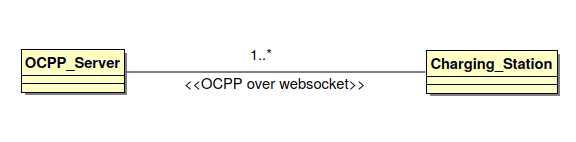
\includegraphics[width=\linewidth]{ocppOverview}
\caption{OCPP overview.}
\end{figure}

\end{center}


\section{Minimal OCPP implementation}
The OCPP protocol supports many use cases which are not required for a basic implementation. The following table \cite{ocpp} shows a minimal subset of OCPP messages required to support basic functionality.\\

\begin{table}[htp]
\caption{Use cases for a basic implementation}
\begin{tabular}{ |p{4cm}|p{3cm}|p{4cm}|p{2cm}| p{1.5cm}|p{1.5cm}|p{1.5cm}|p{1cm}|p{1cm} }
 \hline
Functionality & 
Use Case & 
Messages &
Complete
\\
 \hline
Booting a charge station& B01 - B04& BootNotification & \cellcolor{green} \\
 \hline
Configuring a charge station & B05-B07 & SetVariables, GetVariables, GetReportBase & \cellcolor{green} \\
 \hline
Resetting a charge station& B11-B12 & Reset & \\
 \hline
Authorization Options& One of C01, C02, C04 & Authorize &\\
 \hline
Transaction Mechanism & E01 (one of S1-S6), E02-E03,
E05, E06 (one of S1-S6), E07-
E08, One of E09-E10, E11-E13 & TransactionEvent & \\
 \hline
Availability& G01, G03-G04& ChangeAvailability, StatusNotification &\\
 \hline
Monitoring Events& G05, N07 & NotifyEvent & \\
 \hline
Meter Values & J02 & TransactionEvent & \\
 \hline
Data Transfer& P01-P02 & DataTransfer & \\
 \hline
\end{tabular}
\end{table}

\subsection{Boot Notification}
A high level view of a typical boot notification sequence is given in Figure \ref{fig:SD-B01}.
	\begin{center}
		\begin{figure}[H]
			\label{fig:SD-B01}
			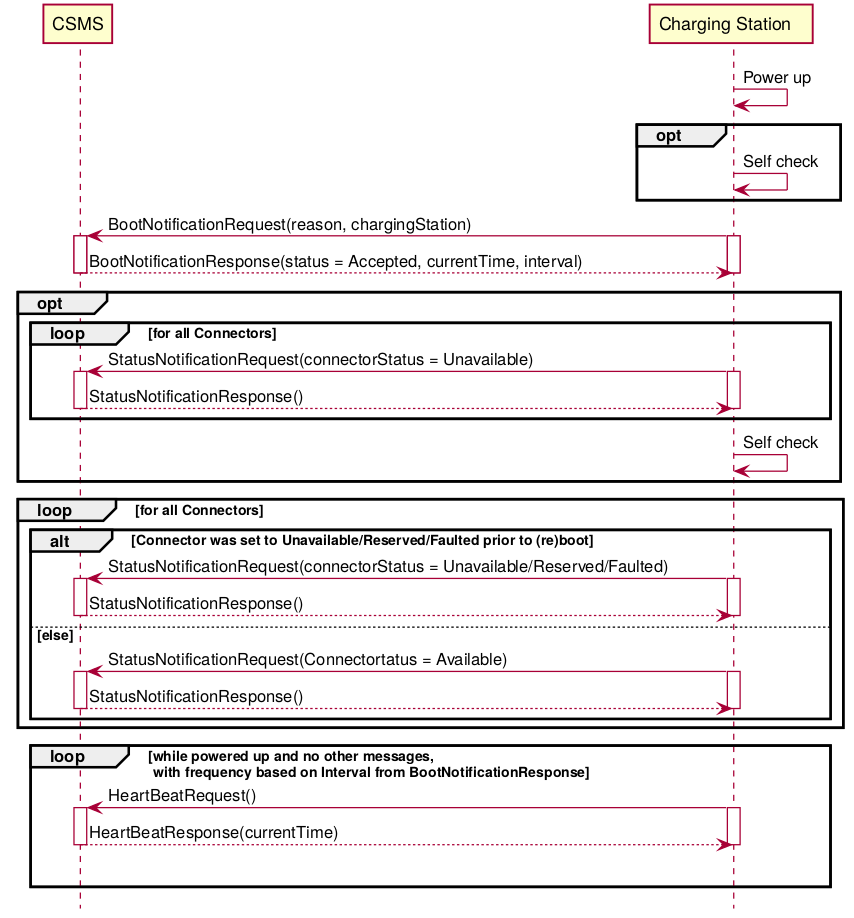
\includegraphics[width=\linewidth]{SD-B01}
			\caption{Cold Booting a Charging Station \cite{ocpp2b}.}
		\end{figure}
	\end{center}

\subsubsection{Implementation}



\chapter{Results and discussion \ldots}

\ldots\ or perhaps the discussion should be a separate chapter.

In any case, you will probably need to include tabulated results.
\tab{tf2} illustrates the use of various \LaTeX\ environments to
include a computer printout (plain text file) in a document.  The
\texttt{verbatim} environment, which encloses the formatted text, is
also useful for program listings.

\chapter{Conclusions}

\section{Summary and conclusions}

\section{Possible future work}
\subsection{Websocket Implmentation}


\appendix

% Chapters after the \appendix command are lettered, not numbered.
% Setting apart the appendices in the table of contents is awkward:

\newpage
\addcontentsline{toc}{part}{Appendices}
\mbox{}
\newpage

% The \mbox{} command between two \newpage commands gives a blank page.
% In the contents, the ``Appendices'' heading is shown as being on this
% blank page, which is the page before the first appendix.  This stops the
% first appendix from be listed ABOVE the word ``Appendices'' in the
% table of contents.

% \include appendix chapters here.

\chapter{Dummy appendix}

\section{Dafny}


\label {dafnybug1}

\begin{verbatim}

https://github.com/dafny-lang/dafny/issues/532
Simulated type set crashes at run-time \#532
An attempt to do a dynamic type test causes a crash when the compiled program is run. This should either be disallowed statically or should compile to good code.

Repro: Here is the output on the program below:

\$ dafny /compile:3 test.dfy
Dafny 2.3.0.10506
test.dfy(17,19): Warning: /!\ No terms found to trigger on.

Dafny program verifier finished with 2 verified, 0 errors
Running...

t.x=5  The given Tr is a C, and c.y=6
t.x=100  Error: Execution resulted in exception: Exception has been thrown by the target of an invocation.
System.InvalidCastException: Specified cast is not valid.
%  at _module.__default+<M>c__AnonStorey0.<>m__0 () [0x00023] in <73b9bd36ee6e47fba3617ec618048be5>:0
%  at _module.__default.M (_module.Tr t) [0x0003b] in <73b9bd36ee6e47fba3617ec618048be5>:0
%  at _module.__default.Main () [0x00058] in <73b9bd36ee6e47fba3617ec618048be5>:0
%  at (wrapper managed-to-native) System.Reflection.MonoMethod.InternalInvoke(System.Reflection.MonoMethod,object,object[],System.Exception&)
  at System.Reflection.MonoMethod.Invoke (System.Object obj, System.Reflection.BindingFlags invokeAttr, System.Reflection.Binder binder, System.Object[] parameters, System.Globalization.CultureInfo culture) [0x00032] in <bb7b695b8c6246b3ac1646577aea7650>:0



And here is the program:

trait Tr {
  var x: int
}

class C extends Tr {
  var y: int
}

class D extends Tr {
  var z: int
}

method M(t: Tr)
  modifies t
{
  print "t.x=", t.x, "  ";
  var s: set<C> := set c: C | c == t;  // this line crashes for the call M(d)
  if s == {} {
%    print "The given Tr is not a C\n";
  } else {
    var c :| c in s;
%    print "The given Tr is a C, and c.y=", c.y, "\n";
    c.y := c.y + 10;
  }
}

method Main() {
  var c := new C;
  var d := new D;
  c.x, c.y := 5, 6;
  d.x, d.z := 100, 102;

  M(c);
  M(d);
  M(c);
}

\end{verbatim}

\label{dafnybug2}
\begin{verbatim}
https://gitter.im/dafny-lang/community?at=5d90c402086a72719e848f24
Bryan Parno
@parno
Mar 14 05:41
We use reference counting via shared_ptr Which means it is possible to create memory leaks if you try hard enough (e.g., via a doubly-linked list). For the latter case, I've been thinking about adding an annotation that a developer could add that would give the compiler a hint that it should use a weak_ptr to break up such cycles, but I haven't gotten around to it yet
\end{verbatim}





Appendices are useful for supplying necessary details or explanations
which do not seem to fit into the main text, perhaps because they are
too long and would distract the reader from the central argument.
Appendices are also used for program listings.

Notice that appendices are ``numbered'' with capital letters, not
numerals.  When the \verb+\appendix+ command in
\LaTeX~\cite[p.\,175]{lamport} is used with the \texttt{book} document
class, it causes subsequent chapters to be treated as appendices.

\chapter{Program listings}

\section{First program}

Some initial explanatory notes may precede the listing.

\section{Second program}

\section{Etc.}

\chapter{Companion disk}

See https://github.com/DanielMcInnes/thesis.git .

\cleardoublepage

\nocite{*}
\bibliographystyle{IEEEannot}
\bibliography{annot}
\end{document}
